% !TeX encoding = UTF-8
% !TeX program = xelatex
% !TeX spellcheck = en_US

\documentclass{cjc}

\usepackage{booktabs}
\usepackage{siunitx}
\usepackage{hyperref}
\usepackage{nicematrix}
\usepackage{algorithm}
\usepackage{algorithmic}
\usepackage{subfigure}
\usepackage{stfloats}
\begin{document}

\title{基于x86多核处理器的高通量多元LDPC码FFT-SPA译码器的实现}
\author{Bertrand Le Gal\footnote{IMS Lab., Univ. Bordeaux, Bordeaux INP, CNRS UMR 5218, France} \and Christophe Jego\footnotemark[1]}

\maketitle

\begin{abstract}
  低密度奇偶校验(LDPC)码是一种众所周知的错误码,常被用于无线通信和卫星通信。
  而通过将LDPC码扩展到高阶伽罗瓦域,能够进一步提高其纠错性能,从而产生了所谓的
  多元LDPC码(NB-LDPC)。而纠错性能改进(CCSDS \citeyear{CCSDS_2014})是国际空间数据系统咨询委员
  会(CCSDS)在下一代上行链路实验规范(CCSDS \citeyear{CCSDS_2014}、\citeyear{CCSDS_2015})
  中采用NB-LDPC码的主要原因。NB-LDPC码对短帧具有较高的纠错效率,因此该码是物联网应用的理想选择。
  然而,这种性能上的增益是以解码计算复杂度为代价的(CCSDS \citeyear{CCSDS_2014}; CondeCanencia etal. \citeyear{comparison_NBLDPC})。
  本文给出了一个x86多核NB-LDPC译码器的实现。与GPU(图形处理单元)设备上最高效的
  工作相比,这一实现FFT-SPA算法的译码器的吞吐量提高了约1.3倍到2.7倍,延迟减少了
  95\%以上,功耗降低了一半。实际上,在x86架构上进行高效的内存映射和计算优化的话,
  可以实现比基于类似实验设置的GPU更高的解码吞吐量。因此,吞吐量效率、低功耗下的
  低处理延迟使得本文所提出的多核方案对于用于CCSDS标准和未来物联网应用中的SDR、
  Cloud-RAN系统中的NB-LDPC译码器的实时实现极具现实意义。\medskip\newline
  \textbf{关键字 }多元LDPC码,FFT-SPA,多核,SIMD,纠错码

\end{abstract}

\section{简介}

  纠错码(ECC)是现代数字通信系统中广泛用于提高系统可靠性的纠错技术。而低密度奇偶
  校验码\cite{gallager_low_1962}由于其接近信道容量的性能,成为了最流行的纠错码之一。
  许多卫星通信标准,如 DVB-S2X \cite{noauthor_dvb_nodate} 或 CCSDS \cite{CCSDS_2011},
  都采用了这种码族。文\cite{davey_low_1998,noauthor_barnault_nodate}提出了将二进制LDPC码扩展到多进制伽罗瓦域
  的方法,以提高纠错性能。这类方法很可能在未来的CCSDS标准中被采用\cite{CCSDS_2015,dolecek_non-binary_2014}。
  事实上,在CCSDS环境中,应用该方法后的纠错增益从1.0 dB提升到了1.3 dB\cite{CCSDS_2015}。
  因此,大量的研究集中在这一新的具有挑战性的代码系列上,例如高效的软件解码器实现\cite{noauthor_wang_nodate,noauthor_andrade_nodate,noauthor_beermann_nodate,andrade_optimized_2014,noauthor_thi_nodate,beermann_gpu_2015,noauthor_pham_nodate,liu_high-throughput_2018}
  或高效的硬件架构设计\cite{boutillon_design_2013,abassi_novel_2017}。
  然而,诸如灵活性、高吞吐量和低延迟等一系列面向未来基于SDR的系统的特性还有待进一步研究。

  ECC 技术通常用计算复杂度来区分。在过去的十年中,ASIC 或 FPGA是首选的实现方法,
  甚至对于地面基带站也是如此。实际上,基于 ASIC 的方案提供了最佳的面积、功耗和吞吐量特性。
  但是,它们的运行时灵活性低,开发周期长。为了解决这一问题,研究了基于FPGA的体系结构设计。
  而这些目标具有计算并行性强和低功耗的优点。然而,基于FPGA的硬件实现也具有有限的灵活性,
  并且设计周期也过长。另一方面,ASIC 和 FPGA 的实现都是基于近似的译码算法,
  这使得架构成本最小化的同时给纠错能力带来了负面影响。

  大规模并行可编程器件在获得很大进步和发展后,已被用于许多纠错码的译码器实现中,
  例如二进制LDPC码\cite{chang_accelerating_2011,falcao_portable_2012,noauthor_wang_nodate-1,li_efficient_2013,lin_high_2014,gal_high-throughput_2016,andrade_survey_2016}
  、NB-LDPC码\cite{noauthor_wang_nodate,noauthor_andrade_nodate,noauthor_beermann_nodate,andrade_optimized_2014,noauthor_thi_nodate,beermann_gpu_2015,noauthor_pham_nodate,liu_high-throughput_2018}
  和极性码\cite{noauthor_gal_nodate,gal_multi-gbs_2015,giard_low-latency_2018}。
  这些软件译码器的设计可达到Mbps或Gbps的吞吐量,也能够提供软件无线电(SDR)\cite{grayver_implementing_2013}
  系统所需的灵活性。

  许多最近的研究工作专注于NB-LDPC译码器在GPU设备上的软件实现\cite{noauthor_wang_nodate,noauthor_andrade_nodate,noauthor_beermann_nodate,andrade_optimized_2014,noauthor_thi_nodate,beermann_gpu_2015,noauthor_pham_nodate,liu_high-throughput_2018}。
  虽然二进制LDPC译码器在GPU和多核目标上的高效实现已经比较理想\cite{chang_accelerating_2011,falcao_portable_2012,noauthor_wang_nodate-1,li_efficient_2013,lin_high_2014,gal_high-throughput_2016,andrade_survey_2016},
  但是NBLDPC码却相去甚远。实际上,NB-LDPC译码算法与二进制LDPC译码算法有很大的不同。
  这意味着以前的优化策略不能直接移植。因此,针对GPU目标,研究人员提出了另外的并行化策略。
  由于解码算法的主要差异,还必须在多核体系结构上重新设计它们。第一批研究\cite{noauthor_andrade_nodate,noauthor_beermann_nodate,andrade_optimized_2014,beermann_gpu_2015,liu_high-throughput_2018}
  集中于在GPU目标上实现具有高纠错性能的NB-LDPC解码算法,用于只关注纠错性能的应用。
  使用5次分层译码迭代后,GPU上的吞吐率从1Mbps提高到了228Mbps。然而,处理延迟显著增加:
  当选择最有效的吞吐量设置时,延迟在21 ms到123 ms不等\cite{liu_high-throughput_2018}。
  第二批研究\cite{noauthor_wang_nodate,noauthor_thi_nodate,noauthor_pham_nodate}
  集中于在GPU设备上实现解码启发式算法。然而,即便有较低的计算复杂度,与基于初始公式的解码吞吐量相比,
  所实现的解码吞吐量仍不可观\cite{noauthor_andrade_nodate,liu_high-throughput_2018}。
  大多数基于GPU的解码器在吞吐量或延迟方面的低性能水平是由GPU的体系结构导致的,
  例如缓慢的全局内存、有限的共享内存等,及其相关的编程模型,这些限制造成实现NB-LDPC
  解码算法极具挑战性。

  本文详细介绍了另一种基于x86多核结构的NB-LDPC译码器的软件实现。本文选择FFT-SPA算法是因为它比最小和或SPA译码算法具有更低的计算复杂度和更高的纠错性能
  \footnote{尽管优化过的SPA和最小和译码器不是本文重点,但仍对其进行了实现和测试。在“实验”一章中有一栏对这些算法进行了性能比较。}。
  x86处理器的编程模型和结构特点与GPU不同。尽管与GPU设备相比,该算法的处理单元较少,
  但它似乎更好地利用了x86多核特性,就像其他ECC码族一样\cite{gal_high-throughput_2016,noauthor_wang_nodate-1,noauthor_cassagne_nodate}。
  此外,该解码器的吞吐量比大多数相关成果都要高\cite{noauthor_andrade_nodate,noauthor_beermann_nodate,andrade_optimized_2014,beermann_gpu_2015,liu_high-throughput_2018}。
  特别是在服务器级x86 CPU上,总能得到更好的吞吐量、延迟和功耗特性。
  为了达到这个性能水平,本文采用了不同的并行化策略和算法优化。实验结果表明,
  所提出的NB-LDPC软件译码器实现方案在吞吐量、延迟和能量消耗方面比基于GPU的实现更具竞争力。
  功耗的降低和低延迟的特性使得该实现更适合于SDR系统。与第一个借助OpenCL语言\cite{noauthor_wang_nodate}
  实现的x86软件解码器实现相比,本文提出的软件解码器实现直接利用了SIMD和多核特性,
  使其比\cite{noauthor_wang_nodate}中给出的x86实现快1000倍以上。

  论文的其余部分组织如下。第 \ref{sec:decoding} 节介绍了NB-LDPC码、FFT-SPA译码算法
  以及在GPU上实现NB-LDPC译码器的相关工作。然后,第 \ref{sec:fftspa} 节详细介绍了
  目标x86多核平台以及我们的并行化和优化方法。最后,在第 \ref{sec:experiment} 节中
  提供了性能分析和与相关工作的横向对比。

\section{NB-LDPC 码的译码}\label{sec:decoding}
\subsection{简介}

  $(N,K)$ NB-LDPC 码是一种由稀疏奇偶校验矩阵 $H$ 定义的线性分组码,其中非零元素属于
  $q\geq2$ \eqref{eq:1} 的伽罗瓦域$\mathbb{GF}(q)$。$H$矩阵的维数为$M{\times}N$,
  其中$M=N−K$是奇偶方程(或校验节点,CN)的数目,N是可变节点(VN)的数目,即码字中
  $\mathbb{GF}(q)$符号的数目。当$H$矩阵中的值$\alpha_{ij}$不为0时,
  $c_j$奇偶方程中就会带有元素$v_i$。第$j$行中非零元素的个数定义为用$d_{c_j}$表示的 CN 度。
  类似地,定义了第$i$列中非零元素的数量作为用$d_{v_i}$表示的 VN 度。

\begin{equation}\label{eq:1}
  \setlength{\arraycolsep}{3pt}
  H=
  \begin{pNiceMatrix}[first-row,first-col]
        & v_{0} & v_{1} & v_{2} & v_{3} & v_{4} & v_{5} & v_{6} & v_{7}\\
    c_0 & \alpha_{00} & \alpha_{10} & \alpha_{20} & 0 & 0 & 0 & 0 & 0 \\
    c_1 & 0 & 0 & 0 & \alpha_{31} & \alpha_{41} & \alpha_{51} & 0 & 0 \\
    c_2 & \alpha_{02} & 0 & 0 & \alpha_{32} & 0 & 0 & \alpha_{62} & 0 \\
    c_3 & 0 & \alpha_{13} & 0 & 0 & \alpha_{43} & 0 & 0 & \alpha_{73} \\
  \end{pNiceMatrix}
\end{equation}

  定义NB-LDPC码的$H$矩阵也可以用Tanner图表示,如图 \ref{fig:1} 所示。

\begin{figure}[htb]
  \centering
  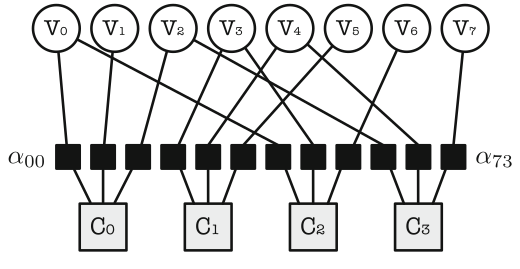
\includegraphics[width=\linewidth]{assets/fig1.png}
  \caption{Eq.\ref{eq:1}中 $H$ 矩阵的Tanner图}\label{fig:1}
\end{figure}

  码字由$x=\{x_0,x_1,\dots,x_{N-1}\}$表示,其中$x_i,i\in[0,N-1]$ 是由 $m=\log_2(q)$
  位表示的$\mathbb{GF}(q)$符号。为了描述等于$\mathbb{GF}$的$q$元素之一的符号$x$的概率$q$,
  使用 q 维 LR 向量。$x_i$的第 $a$ 个符号元素的概率由 $p_i(a),a\in[0,q-1]$ 表示。

  集合$\Psi(c_j)$表示奇偶校验方程$c_j$中包含的$x$个$d_{c_j}$符号。同样,集合$\Psi(x_i)$
  包含了含有符号$x_i$的$d_{v_i}$校验方程。排除由符号$/$表示,例如,$\Psi(x_i)/c_j$表示
  除$c_j$外的$\Psi(x_i)$检验方程组。

  与二进制 LDPC 译码类似,NB-LDPC 译码基于消息传递算法执行。最佳纠错性能是通过执行
  Sum-Product算法\cite{carrasco_non-binary_2008}(SPA)或其等效公式(如FFT-SPA\cite{carrasco_non-binary_2008})获得的。
  FFT-SPA 解码算法的优点之一,是由于去除消息卷积而使得处理 CN 的计算复杂度降低。
  这种改进是在不影响解码性能的情况下获得的,因为它们在数学上是等价的\cite{comparison_NBLDPC}。
  此外,如在\cite{noauthor_andrade_nodate}中强调并在\cite{carrasco_non-binary_2008}中演示的,
  大多数$\mathbb{GF}(q)$域的解码操作都被转移到了$\mathbb{R}$,以便于实现。

  算法1提供了用于水平分层解码调度的形式化FFT-SPA解码算法\cite{beermann_gpu_2015,liu_high-throughput_2018,noauthor_hocevar_nodate}。
  与基于泛洪的调度相比,它有助于:(i)在提供类似的纠错性能的同时加倍收敛速度;
  (ii)减少解码器的内存占用。这些特性使得这种计算调度在软件\cite{noauthor_thi_nodate,beermann_gpu_2015,noauthor_pham_nodate,liu_high-throughput_2018}
  和硬件\cite{boutillon_design_2013,abassi_novel_2017}实现中都很流行。

\begin{algorithm}[htb]
  \begin{algorithmic}[1]
    \STATE \textbf{Step 1}: 初始化
    \STATE $p_i(x)=p(v_i=x|y_i)$
    \STATE $m^0_{ji}(x)=1$
    \STATE $\vartriangleright$ 进行 $iter_max$ 次解码迭代
    \FORALL{$t=1\rightarrow(iter\_max)$}
      \STATE \textbf{Step 2}: 轮询 NB-LDPC 码中的所有 CN
      \FORALL{$j{\in}C$}
        \STATE$\vartriangleright$ 计算接收到的消息 $m_{ij}$
        \FORALL{$i\in\Psi(j)$}
          \STATE $m_{i j}^{t}(x)=\left(\sum_{x \in \mathbb{G} \mathbb{F}} m_{j i}^{t-1}(x)\right) \times\left(\frac{p_{i}(x)}{m_{j i}^{t-1}(x)}\right)$
          \STATE $M^t_{ij}=\Theta_{\alpha_{ij}}(m^t_{ij})$
          \STATE $\tilde{M^t_{ij}}=FFT(M^t_{ij})$
        \ENDFOR
        \STATE$\vartriangleright$傅里叶域中累乘概率
        \FORALL{$i\in\Psi(j)$}
          \STATE $\tilde{M}_{j i}^{t}=\prod_{i^{\prime} \in \Psi(j) / i} \tilde{M}_{i^{\prime} j}^{t}$
        \ENDFOR
        \STATE$\vartriangleright$计算输出的消息 $m_{ij}$
        \FORALL{$i\in\Psi(j)$}
          \STATE $M^t_{ji}=FFT^{-1}(\tilde{M^t_{ji}})$
          \STATE $m^t_{ji}=\Theta^{-1}_{\alpha{ij}}(M^t_{ji})$
        \ENDFOR
        \STATE$\vartriangleright$更新符号概率
        \FORALL{$i\in\Psi(j)$}
          \STATE $p_i(x)=p_i(x)\times(\frac{m^t_{ji}(x)}{m^{t-1}_{ji}(x)})$
        \ENDFOR
      \ENDFOR
    \ENDFOR
    \STATE\textbf{Step 3}: 符号硬判
    \FORALL{$i\in{V}$}
      \STATE $\hat{v}_{i}=\arg \max \left(p_{i}(x)\right)$
    \ENDFOR
  \end{algorithmic}
  \caption{ 水平 TDMP FFT-SPA 算法}
  \label{alg:1}
\end{algorithm}

  该算法可以概括为三个主要步骤。首先,使用 $y_i$ 信道信息计算 $N$ 个接收符号 $p_i$ 的概率
  (算法1:行2)。对于每个符号 $p_i$,估计每个元素$x\in\mathbb{GF}(q)$的概率。
  其次,对 $H$ 矩阵中的所有 CN 依次求值(算法1:行7:27)。对于 CN 计算,首先动态
  计算从 VN 到 CN 的 $m_{ij}$ 消息。然后,生成 $m_{ji}$ 消息并更新每个符号
  $p_i(x)$ 的概率。最后,对于每个 $p_i(x)$,选择具有最高概率$p_i(x)$ 的符号
  $\tilde{v}_v$(算法1:行30:32)。

  重复包括顺序处理 CN 的第二步,直到达到最大迭代次数或获得有效码字为止。CN 处理可扩展为7个基本阶段:
\begin{enumerate}
  \item 从 VN 到 CN 的消息 $m^t_{ij}(x)$ 是根据当前 VN 值($p_i(x)$)和从上一次
  迭代中从 CN 到 VN 的消息($m^{t-1}_{ji}(x)$)进行动态计算。
  \item 消息 $m_{ij}$ 在 $\mathbb{GF}$ 域中与来自 $H$ 矩阵的 $\alpha_{ij}$ 值相乘。
  此操作等效于受 $\alpha_{ij}$ 约束的数据置换,表示为 $\Theta_{\alpha_{ij}}$。
  \item 然后使用 $FFT$ 变换操作,$M_{ij}$ 消息值被转换到傅里叶域。
  \item 在$\tilde{M}_{ij}$消息值之间的进行一组标量乘法产生 CN 到 VN 消息。
  \item 通过 $FFT^{-1}$ 变换操作,消息值被转回概率域。 
  \item 消息 $M_{ji}$ 在 $\mathbb{GF}$ 域中除以第 2 阶段中使用的 $\alpha_{ij}$ 值。
  \item 最后,根据计算出的 $m^t_{ji}(x)$ 值来更新符号概率 $p_i(x)$。
\end{enumerate}

  在解码过程中,解码器只需要存储 $N$ 个 $p_i$ 元素和 $M\times{d_{c_j}}$ 个 $m_{ji}$ 元素。
  实际上,在第 $t−1$ 次迭代中用于存储的元素 $m^{t-1}_{ji}$ 的内存可以被重用于
  在第 $t$ 次迭代中存储元素 $m^t_{ji}$。注意,元素 $p_i$ 和 $m_{ji}$ 本质上由 $q$ 元素构成。

\subsection{相关工作}
  
  为了提供实现灵活性和高吞吐量性能,最近的许多研究都集中在将 NB-LDPC 解码器在 GPU 设备上实现\cite{noauthor_wang_nodate,noauthor_andrade_nodate,noauthor_beermann_nodate,andrade_optimized_2014,noauthor_thi_nodate,beermann_gpu_2015,noauthor_pham_nodate,liu_high-throughput_2018}。
  这些研究的目的是利用 GPU 设备提供的大量计算并行度来达到高吞吐量,就像之前对二进制
  LDPC 解码所做的那样\cite{li_efficient_2013,lin_high_2014,gal_high-throughput_2016}。
  实际上,为了使软件方案适用于数字通信系统仿真或 SDR 目的,必须解决灵活性、吞吐量、延迟和功耗效率等问题。

  第一批工作\cite{noauthor_andrade_nodate,noauthor_beermann_nodate,andrade_optimized_2014,beermann_gpu_2015,liu_high-throughput_2018}
  专注于基于 SPA 的算法,以提供高纠错性能。为了降低解码过程的计算复杂度,FFT-SPA \cite{noauthor_andrade_nodate}
  解码算法是首选。实际上,在 CN 处理中引入的 FFT 运算将 SPA 算法的卷积运算转化为一组标量项的乘积。
  CN 处理的计算复杂度原来是$O(M\times3\times(d_c−2)\times2^{2{\times}m})$,现在降低
  到$O(M\times{d_c}\times{m}\times2^{m})$\cite{declercq_decoding_2007}。
  \cite{noauthor_andrade_nodate}中报告的第一个基于 GPU 的实现在执行 10 次泛洪迭代时,
  $\mathbb{GF}(256)$ NB-LDPC 码的吞吐量在 0.5 到 1.6 Mbps 之间。由于 FFT 处理中计算并行性的降低,
  所以 $q$ 值较低时吞吐量也较低。这实际上限制了 GPU 核心的使用率,从而进一步
  限制了解码器的全局效率。\cite{noauthor_beermann_nodate}中也报告了类似的结论。
  注意,这项工作的第一个目标是支持不规则的 NB-LDPC 码。在\cite{beermann_gpu_2015}中,
  详细介绍了基于 FFT-SPA 算法分层公式的 NB-LDPC 解码器的实现。与\cite{noauthor_beermann_nodate}
  中提到的方法相比,它增加了解码吞吐量,从而实现了等效的纠错性能。
  然而,对于 $\mathbb{GF}(16)$ 到 $\mathbb{GF}(256)$ NB-LDPC 码,所测量的解码
  吞吐量仍然低于 0.5 Mbps。最近,在\cite{liu_high-throughput_2018}中提出了一种高效的
  基于 GPU 的解码器实现。在考虑 GPU 特性的基础上,找到了 FFT-SPA 译码算法的有效实现。
  基于分层的调度与高端 GPU 设备的组合使得能够针对 $\mathbb{GF}(16)$ NB-LDPC 码获得
  228 Mbps 的峰值吞吐量和 123 ms 的处理延迟。

  第二批工作\cite{noauthor_wang_nodate,noauthor_thi_nodate,noauthor_pham_nodate}
  集中于 SPA 解码算法的简化版本。不过,SPA 和 FFT-SPA 解码算法由于其高计算复杂度
  而不满足硬件结构设计约束。此后,为了便于 NB-LDPC 译码器的硬件实现,提出了一些
  低复杂度的译码算法:MinSum\cite{declercq_decoding_2007}、Min-Max\cite{declercq_decoding_2007}
  和 Extended Min-Sum\cite{noauthor_voicila_nodate}。在这些译码算法中,$\mathbb{R}$中
  的乘法和除法运算被转换成加法、减法和最小/最大运算。一些基于 GPU 的实现\cite{noauthor_wang_nodate,noauthor_thi_nodate,noauthor_pham_nodate}
  侧重于 min-max 解码技术。事实上,低计算复杂度似乎更好地在GPU设备上实现。需要注意的是,
  与基于 SPA 的算法相比,min-max 算法对纠错性能也有负面影响。然而,即使具有较低的计算复杂度,
  对于 $\mathbb{GF}(32)$ NB-LDPC 码,GPU 实现也未能达到高于 0.7 Mbps 的吞吐量。
  这种效率问题来自于 CN 计算中涉及的卷积式处理。

  总的来说,在 GPU 实现的相关工作表明,NB-LDPC 译码过程具有较高的计算并行度。
  因此,,它可以借助多核实现加速。然而,与 GPU 设备相关联的架构约束和编程模型似乎
  限制了 NB-LDPC 解码器在解码吞吐量和延迟方面的实现效率。因此,在本文中,我们重点
  讨论了这样一个多核体系结构,它提供了不同的编程模型和其他体系结构约束。实验结果表明,
  NB-LDPC 译码算法的计算并行度非常适合 x86 处理器。

\section{FFT-SPA 算法实现}\label{sec:fftspa}
\subsection{选定的多核架构}

  多核设备(例如 x86 或 ARM 处理器)提供足够当前的处理资源,以达到 Mbps 或 Gbps 吞吐量性能。
  如二进制 LDPC 码\cite{gal_high-throughput_2016,gal_high-throughput_2015}解码所示,
  它们应该适用于大多数 SDR 系统。所有的现代处理器都提供单指令多数据(SIMD)功能,
  使得在不同的数据集上同时执行 $Q$ 个相同的计算。例如,在当前的 x86 处理器中,
  使用 AVX2 配置,可以用一条指令处理 $Q=8$ 浮点计算。注意,根据功能单元的使用情况,
  时钟周期可以触发多条指令。目前,x86 处理器内核最多可以并发执行 6 条指令。这种
  并行化方法主要适用于不需要条件语句或分支语句的情况下,大量数据需要相同处理的计算序列。
  此外,还可以使用多指令多数据(MIMD)功能。它为不同的计算序列或程序在不同的数据集
  上并行执行提供了机会。因此,它使得并行帧处理成为可能。下一节将详细介绍
  利用 SIMD 和 MIMD 特性提出的 FFT-SPA 实现和优化选择\footnote{实现NB-LDPC 译码器的源代码将会在 GitHub 上开源}。

\subsection{并行化策略}

三种主要的SIMD并行化策略可以加速基于MP的算法:
\begin{itemize}
  \item $S_1$ 策略包括并行解码多个帧,如\cite{gal_high-throughput_2016,gronroos_efficient_2012}
  中的二进制LDPC解码器。它提供了处理和内存访问规则,从而提高了吞吐量性能。尽管如此,
  它依然引入了处理延迟(至少是$Q$倍)和巨大的内存占用。
  \item $S_2$ 策略包括跨 CN 内核的并行计算,例如并行处理 $Q$ 个 CN 内核。该策略缺乏内存访问规则性,
  需要对 CN 内核进行特殊的调度。其实,并行执行的 CN 可以访问不同的 VN 元素。
  \item $S_3$ 策略包括对单个CN内核的并行计算。对于二进制LDPC解码器的软件实现,
  由于CN元素的计算复杂度较低,$S_3$策略被丢弃\cite{gal_high-throughput_2016}。
  不过,对于NB-LDPC译码算法,由于$\mathbb{GF}(q),q\geq{Q}$,CN核的计算复杂度很高,
  并且内存访问是规则的。因此,它使$S_3$策略更为合适。
\end{itemize}

  为了获得最佳的灵活性、吞吐量和延迟平衡,本文放弃了$S_1$和$S_2$并行化策略。
  由于对于所有的NB-LDPC码,不可能实现避免VN访问冲突的CN重排步骤。所以只研究了$S_3$策略。

  表\ref{tab:1}总结了在水平调度计算时FFT-SPA解码算法的CN处理的计算复杂度(算法1)。
  执行每个基于分层的CN处理所需的标量计算的数量由$d_c$归一化。因此,
  它表示的是VN元素所需的标量计算的数量。我们可以注意到整体时间和空间复杂度取决于$\mathbb{GF}$阶数。
  $\mathbb{GF}$阶为$2^m$,一般$m\geq4$。这一属性与SIMD处理器特性十分契合,
  因为SIMD支持$Q$个处理单元,其中$Q$为2的幂。例如,INTEL AVX2 单元能够并行处理$Q=8$的浮点数。
  因此,$m\geq3$ 的NB-LDPC码应能有效地利用SIMD并行化特性。在表\ref{tab:2}中,
  涉及常规计算和内存访问的处理用蓝色表示。这些处理能够加快$Q$倍。红色的处理任务
  对应于由于数据依赖性或不规则的内存/计算序列而导致加速较少的计算。从算法的角度来看,
  FFT-SPA算法的特性似乎很适合x86多核并行化特性。

\begin{table}[htb]
  \caption{\\根据$d_c$归一化后的 CN 处理时间复杂度估计及并行可能性}
  \label{tab:1}
  \setlength\tabcolsep{3pt}% 调整列间距
  \begin{tabular}{cccccc}
    \toprule
    算法1 & 处理任务 & 加/减 & 乘 & 除 & ECN \\
    \midrule
    L.10  & 消息处理 & - & - & \blue{$q$} & - \\
    L.10  & 消息归一化 & \red{$q-1$} & - & \blue{$q$} & - \\
    L.11  & $\mathbb{GF}$中的累乘 & - & - & - & - \\
    L.12  & $FFT$ 处理 & \red{$q.\log_2(q)$} & - & - & - \\
    L.20  & $FFT^{-1}$ 处理 & \red{$q.\log_2(q)$} & - & - & - \\
    L.21  & $\mathbb{GF}$中的除法 & - & - & - & - \\
    L.25  & 更新 VN 值 & - & \blue{$q$} & \blue{$q$} & - \\
    L.16  & 频域中的 CN & - & - & - & \red{$3.(d_c-2)$} \\
    -     & ECN & - & \blue{$q$} & - & - \\
    \bottomrule
  \end{tabular}
\end{table}

\begin{table}[htb]
  \caption{\\根据$d_c$归一化后的 CN 处理空间复杂度估计及并行可能性}
  \label{tab:2}
  \setlength\tabcolsep{4.5pt}% 调整列间距
  \begin{tabular}{ccccc}
    \toprule
    算法1 & 处理任务 & 加载 & 保存 & 存储的数据 \\
    \midrule
    L.10  & 消息处理 & \blue{$2.q$} & \blue{$q$} & $q$ \\
    L.10  & 消息归一化 & \blue{$q$} & \blue{$q$} & $2.q$ \\
    L.11  & $\mathbb{GF}$中的累乘 & \red{$q$} & \blue{$q$} & $q$ \\
    L.12  & $FFT$ 处理 & \blue{$q$} & \blue{$q$} & $q.\log_2(q)$ \\
    L.20  & $FFT^{-1}$ 处理 & \blue{$q$} & \blue{$q$} & $q.\log_2(q)$ \\
    L.21  & $\mathbb{GF}$中的除法 & \red{$q$} & \blue{$q$} & $q$ \\
    L.25  & 更新 VN 值 & \blue{$3\times{q}$} & \blue{$q$} & $q$ \\
    L.16  & 频域中的 CN & - & - & $3q.(d_c-2)$ \\
    -     & ECN & \blue{$2.q$} & \blue{$q$} & $q$ \\
    \bottomrule
  \end{tabular}
\end{table}

  考虑到解码过程的空间复杂度,FFT-SPA 解码算法需要存储$p_i$和$m_{ji}$数据。
  两个集合的每个元素都由$q$个浮点数组成,每个浮点数需要4个字节。因此,在常规 NB-LDPC 码
  的 FFT-SPA 解码器实现中,存储器占用($F$)可以通过以下公式计算(以字节为单位):
  $$F=4\times{q}\times(N+M\times{d_c})$$

  我们选择的帧内并行化策略,将解码器的内存占用限制为低于INTEL处理器 L2 或 L3 内存
  缓存大小的级别(请参阅第 \ref{sssec:experiment11} 节)。而有关解码过程的数据存储要求则非常低,
  如表 \ref{tab:2} 所示。实际上,在处理过程中,除用于FFT计算的临时变量外,要存储的临时变量数目等于$q\times{d_c}$。
  对于 FFT 计算,对临时变量生存期的分析表明,当临时变量变得无用时,内存共享是可能的。
  这能够将存储需求降低到约$3\times{q}$。当$q\leq64$时,SIMD处理器寄存器需要提供足够的存储容量,
  以避免堆栈内存的使用。对于更高阶的$\mathbb{GF}$,需要使用堆栈内存。然而,所需的内存量很低,
  并且必须能提供快速存取的处理器一级内存缓存。解码器的低内存占用和少量的临时变量
  使得通过最小化全局内存访问来实现有效利用内存缓存变得可能。

  合理的内存需求和计算并行化潜力表明INTEL多核体系结构较适合FFT-SPA算法的实现。
  下面详细介绍了译码算法中各个处理任务的实现和优化。

\subsection{实现方案选择与优化}

  软件实现严格遵循算法1中的描述。算法1中的每一行都对应一个由数个原子操作组成的函数。
  这些原子操作包含一个或多个SIMD内部函数,具体取决于操作复杂度和$\mathbb{GF}$阶数。
  在本小节中将全面解释处理实现的关键点。

\subsubsection{内存管理说明}

  高效的内存访问管理和较低的解码器内存占用是在x86目标上实现高性能的主要标准之一。
  实际上,它们通过可以忽略不计的内存访问时间,使利用内存缓存成为可能。与GPU的工作
  (例如\cite{noauthor_beermann_nodate,andrade_optimized_2014})相反,不必为了避免或
  减少由于内存访问冲突造成的运行时惩罚,而去指定所谓2D或3D数据结构。x86体系结构的
  计算并行度低于GPU设备,但它们不涉及对内存元素的硬访问限制。

  在当前的实现中,数据集存储在两个一维数组中。第一个专用于$N$个 $p_i$元素,
  第二个存储$M\times{d_{c_j}}m_{ji}$消息。$p_i$元素根据它们的 $v$ 的下标连续存储,
  例如$\{p_0,p_1,\dots,p_{N−1}\}$。$m_{ji}$元素是根据它们在 CN 内核中的使用顺序存储的。
  例如,当元素$c_0$连接到$\{p_0,p_5,p_9\}$,$\{m_{0,0},m_{0,5},m_{0,9}\}$被消耗。
  每个$p_i$和$m_{ji}$元素由$q$个值组成,这些值在$\mathbb{GF}$域下线性存储。

  根据这种内存映射,并行化策略$S_3$在解码过程中不会产生任何未对齐的内存访问
  ($\mathbb{GF}$乘法和除法步骤除外)。其实,与二进制结构相反,$H$结构引入的
  数据交织过程不是问题。NB-LDPC码将$\mathbb{GF}$元素管理为有$2^m$个元素的数组,
  并可以通过SIMD进行有效管理。因此,在解码过程中对元素的访问(例如,算法1:行10和25)
  相当于从存储器中读写$2^m$对齐的值。故二进制LDPC解码器实现中涉及的聚集和分散的
  存储器访问惩罚不再存在。

\subsubsection{消息\texorpdfstring{$m_{ij}$}{mij}的生成与\texorpdfstring{$p_i$}{pi}的更新}

  在解码过程中,需要连续处理 CN 以避免算法级的 VN 访问冲突管理。在开始 CN 处理时,
  要先计算从 VN 到 CN($m_{ij}$)的消息(算法1:行10)。计算包括将 $p_i(x)$ 除以
  先前的 $m_{ji}(x)$ 值,然后归一化为$q$个$m_{ij}$元素之和。矢量元素$m_{ji}(x)$和
  $p_i(x)$在$\mathbb{GF}$域中排序,以便于内存的存取和划分。而借助SIMD功能,
  它们可以直接执行。$m_{ij}(x)$的和是动态计算的。最后进行水平求和,就能得到归一化因子。
  由于SIMD除法指令比乘法指令慢得多,所以会对归一化因子取倒数。这样就能用乘法运算更新
  所有$m_{ij}(x)$的值。

  在该过程结束时,必须根据计算出的$m_{ji}(x)$值更新$p_i(x)$值(算法1:行25)。
  由于元素的$\mathbb{GF}$阶数相同,剩余的乘法运算可以有效地用SIMD实现。此外,
  在处理器寄存器中更新$p_i(x)$值的同时,定位并选择最佳候选符号$\tilde{v}_i$,
  以加速当前解码迭代结束时停止准则的计算。

  当$q\geq8$时,这两个处理阶段十分受益于SIMD特性,因为它们的内存访问总是对齐的,
  而且计算中会规律性地填充SIMD管道以减少计算延迟。

\subsubsection{\texorpdfstring{$\mathbb{GF}$}{GF}域中的乘除法}

  在生成$m_{ij}$消息后且在涉及 CN 计算的$p_i$更新之前,必须根据$H$矩阵的$\alpha_{ij}$
  值来变换$m_{ij}$和$M_{ji}$消息向量的元素(算法1:行11和21)。$\mathbb{GF}$中涉及计算和
  未对齐内存访问的这些操作可以转换为离线预计算数据重新排序操作。这些操作在运行时不使用符号位置计算。
  但数据重新排序仍然涉及$2^m$个未对齐的内存访问。

  得益于x86 SIMD指令集,这些未对齐的内存访问可以以矢量化的方式实现。
  注意,它会产生一定的延迟开销。幸而SIMD gather指令能帮助我们从内存基址和一组32比特地址偏移量
  中读取32比特浮点数。$\mathbb{GF}(8)$和$\mathbb{GF}(16)$乘法函数的源代码如图 \ref{fig:2} 所示。
  首先,对于$\mathbb{GF}(8)$中的乘法,根据$\alpha_{ij}$值(图\ref{fig:2},行2)
  计算存储了用于数据重新排序的$q$个预计算右值的存储器地址。为追求效率,这$q$个$\alpha$值
  的$q$个内存偏移量被存储在了$q\times{q}$个元素的内存数组中,其中每个元素为32比特。
  首先我们存储与$\alpha_0$相乘所需的$q$个内存偏移量。然后,连续存储$q$个$\alpha_1$内存的偏移量,
  以此类推。这样,要加载右值的内存偏移量以同$\alpha$相乘,可以像$addr_{\alpha}=base\_addr+q\times\alpha$
  这样计算内存偏移基址。一旦计算出内存偏移地址,内存偏移就被加载到SIMD寄存器中
  (图\ref{fig:2},行3)。然后,使用SIMD gather指令执行实现$\mathbb{GF}(8)$乘法的
  伪随机存储器访问(图\ref{fig:2},行4)。此指令结束时,R1寄存器中存储的消息值就被正确排序了。
  最后,消息向量($M_{ij}$)被存储回内存中(图\ref{fig:2},行5)。除了gather指令外,
  整个SIMD进程管理对齐的内存访问。
  
\begin{figure}
  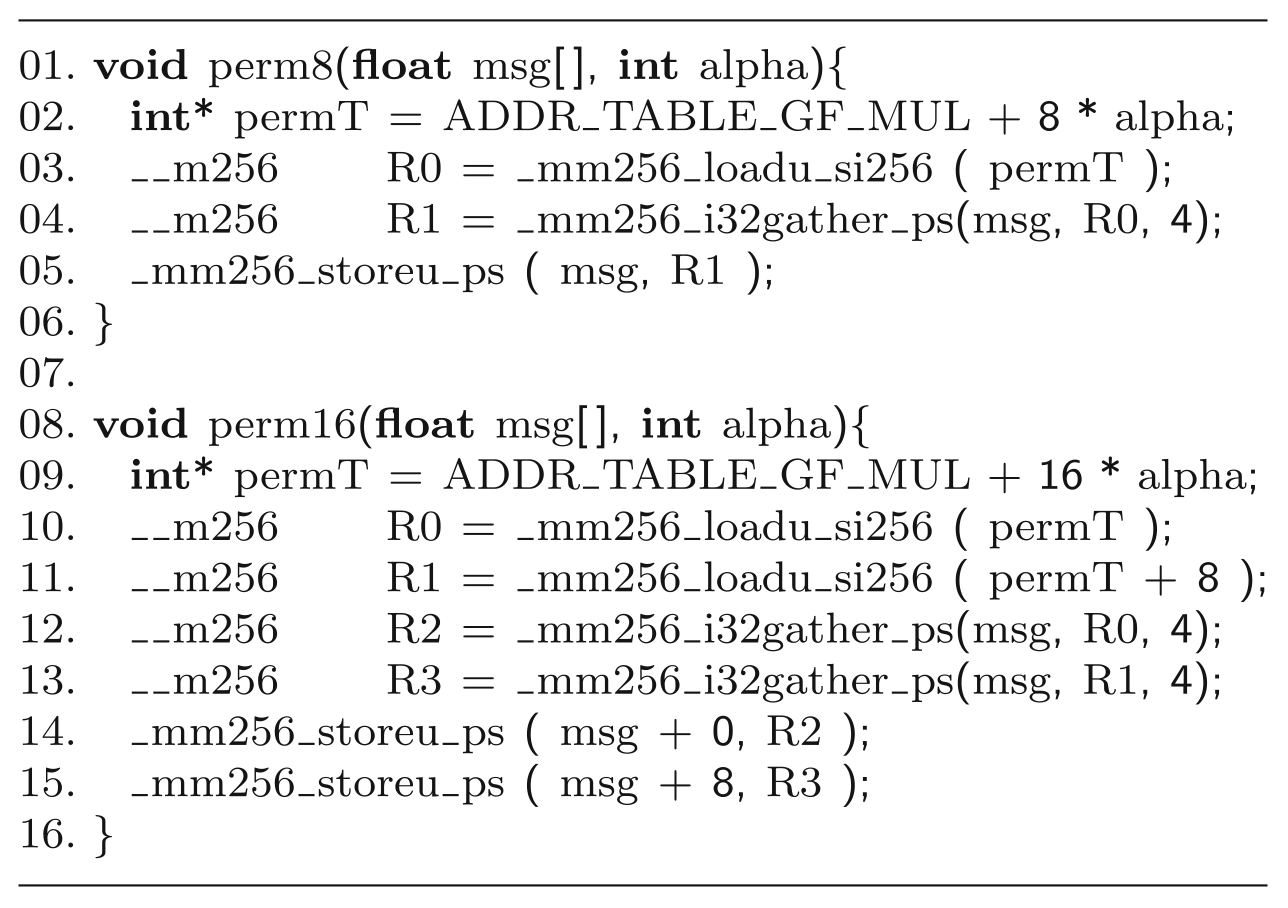
\includegraphics[width=\linewidth]{assets/fig2.png}
  \caption{
    针对 AVX2 优化的$\mathbb{GF}(8)$和$\mathbb{GF(16)}$译码器中的置换函数源代码。
    TABLE\_GF\_MUL 是存储了 $q\times{q}$ 预计算偏移量值数组的内存基地址。
  }\label{fig:2}
\end{figure}

  对于$\mathbb{GF}(16)$乘法,操作是相似的。不过由于要重新排序的$M_{ij}$向量值
  是$\mathbb{GF}(8)$使用的值的两倍,因此操作的数量增加了一倍。对于更高阶数的伽罗瓦,
  过程是相同的。

\subsubsection{域变换}

\begin{figure*}[hbp] % figure* 下不用stfloats的话只有 tp 有效
  \centering
  \subfigure{
    \begin{minipage}{0.45\linewidth}
      \centering
      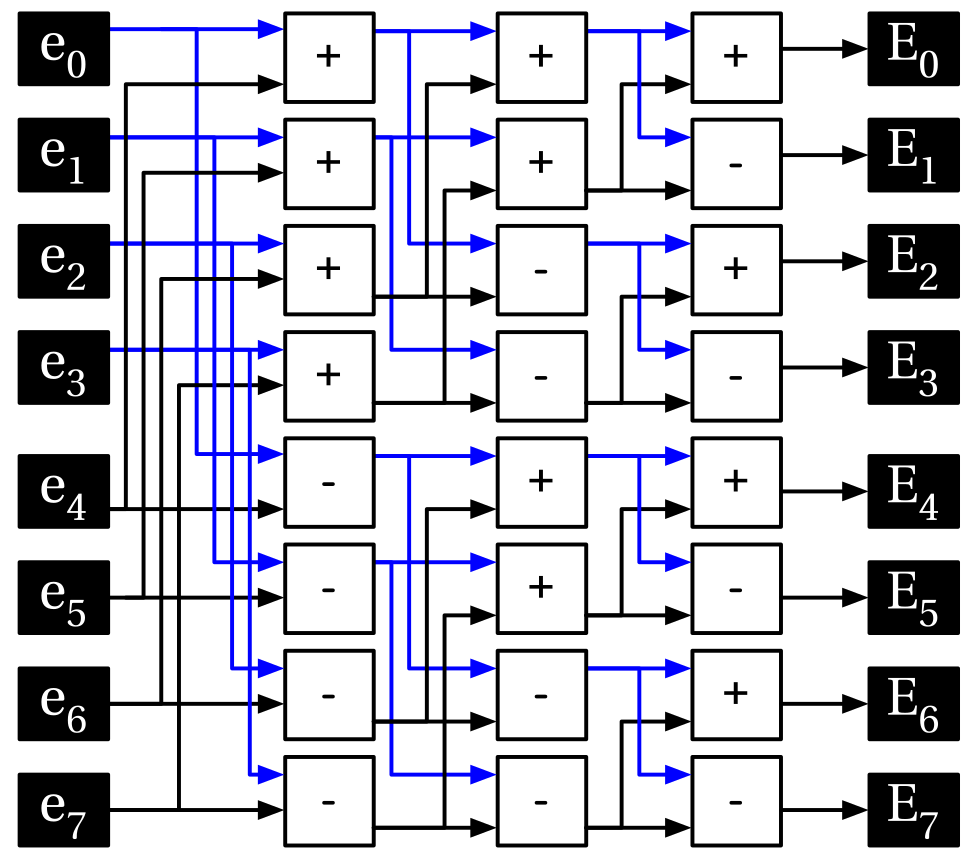
\includegraphics[width=\linewidth]{assets/fig3a.png}
    \end{minipage}
  }
  \subfigure{
    \begin{minipage}{0.45\linewidth}
      \centering
      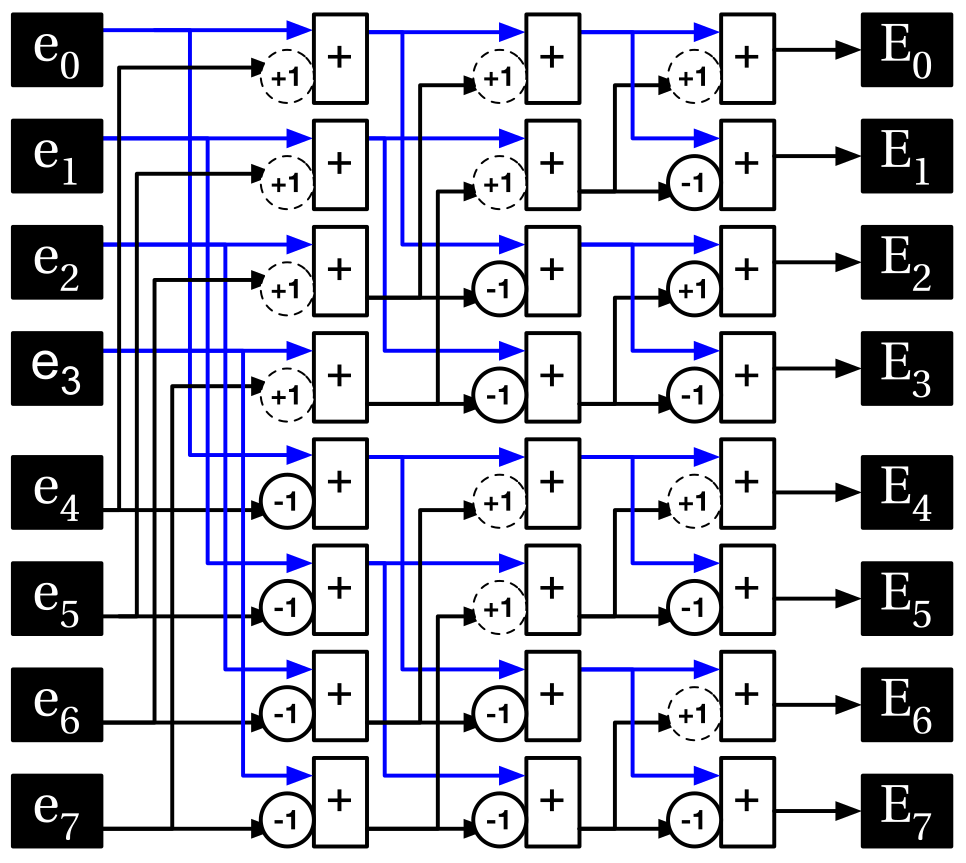
\includegraphics[width=\linewidth]{assets/fig3b.png}
    \end{minipage}
  }
  \caption{
    \textbf{a}:$FHT_{\mathbb{GF}(8)}$过程的原始算法;
    \textbf{b}:$FHT_{\mathbb{GF}(8)}$ 过程的修改后的算法。
  }
  \label{fig:3}
\end{figure*}

  根据\cite{noauthor_andrade_nodate}中的结果,NB-LDPC译码过程的吞吐量瓶颈是傅立叶域变换。
  它抛弃了CN处理中的卷积计算,但仍然有着密集的计算。在\cite{noauthor_andrade_nodate}中,
  选择了快速阿达玛变换(FHT),因为它的计算复杂度有限,并且只需要简单的运算(加法和减法),
  而不影响纠错性能。加法和减法按照图 \ref{fig:3}a 所示的$FHT_{\mathbb{GF}(8)}$蝶形图执行。在这个数据流图中,
  $e_i$是$FHT_{\mathbb{GF}(8)}$的输入,$E_i$是处理的输出,并且处理是标量操作。

  该算法由3组8个可并行执行的计算组成。不过,它并不对SIMD友好,因为它是由加法和减法组成的,
  而SIMD编程模型不支持这种并行性。SIMD处理后的总值必须只经过同一种操作(加法或减法)。

  因此,我们修改了原始$FHT$算法来满足这一SIMD约束。新的算法中,减法被加法代替,
  而一个操作数被取相反数,以保持$FHT$算法功能。处理后的新算法如图 \ref{fig:3}b 所示,
  其中符号反转由−1乘法表示,不变的操作数则乘以1。尽管这种新的公式需要乘法,但它提供了
  规则的运算组,这使其能从SIMD特性中获益。注意,为了实现效率,乘法运算被异或运算取代。
  在二进制掩码下,异或和乘法效果相同。

  图 \ref{fig:4} 提供了对 AVX2 优化的 $FHT_{\mathbb{GF}(8)}$和$FHT_{\mathbb{GF}(16)}$函数源代码。
  其中$m_0$、$m_1$和$m_2$是预先计算的256位二进制掩码,用于反转浮点数符号。代码中寄存器
  的数量有限,且执行的指令具有较低的处理延迟。把输入的内存加载和存储结果时的内存写入算在内的话,
  实现$FHT_{\mathbb{GF}(8)}$处理需要十几条指令。INTEL IACA工具
  \footnote{该工具依据延迟估计,提供了一个处理延迟的理想估计,但不含内存读写惩罚。不过,该工具还提供了指令级的并行和处理瓶颈等方面的有用信息。}
  估计此任务的处理延迟为15个时钟周期。

\begin{figure}
  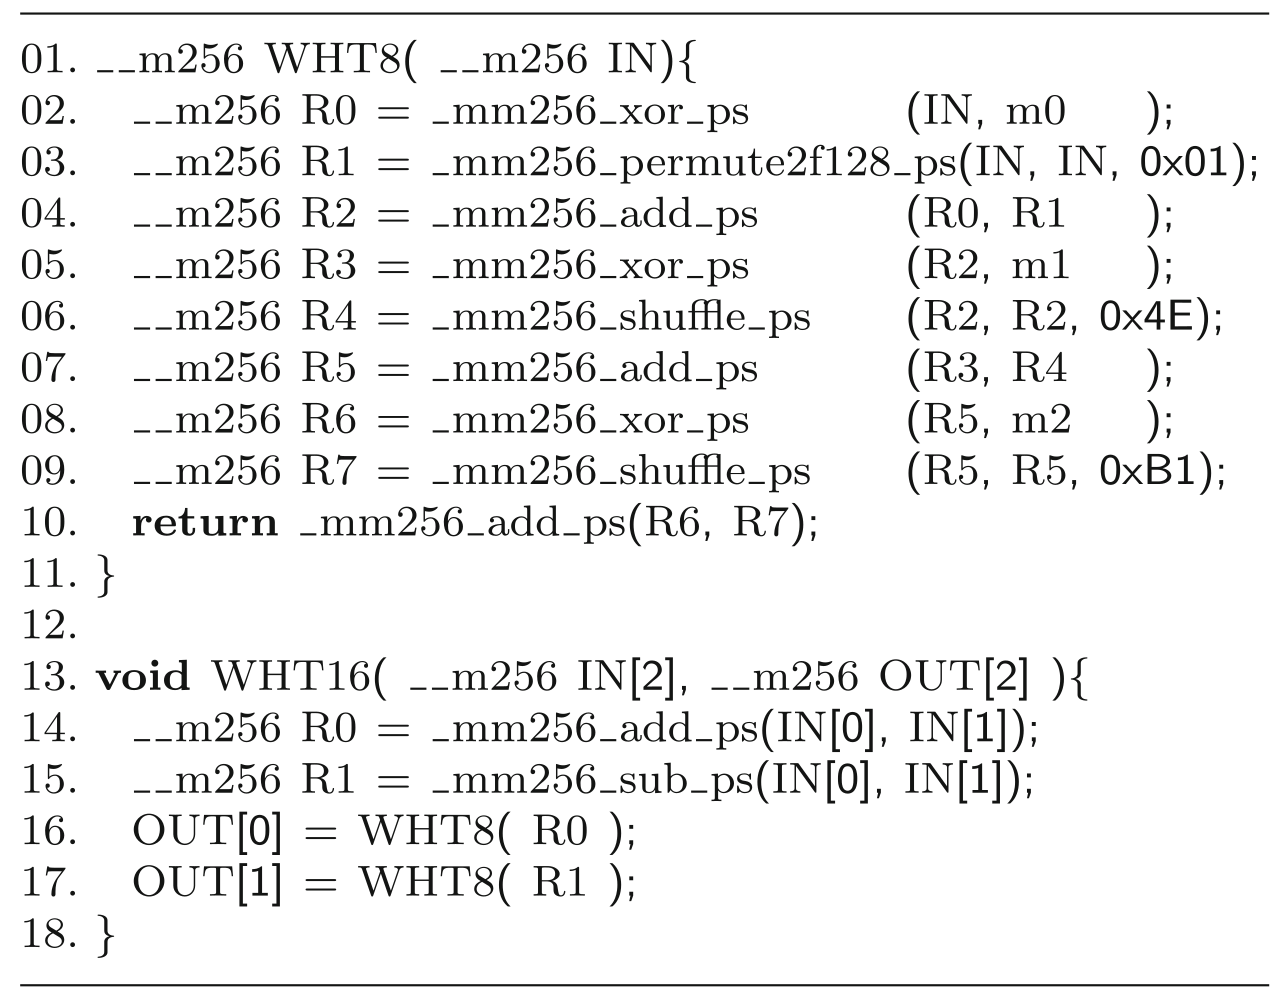
\includegraphics[width=\linewidth]{assets/fig4.png}
  \caption{
    $\mathbb{GF}(8)$和$\mathbb{GF(16)}$译码器中 FHT 函数的源代码。
  }\label{fig:4}
\end{figure}

  更高阶的FHT通过分层分解该处理来获得。$FHT_{\mathbb{GF}(16)}$处理需要两个SIMD加法、
  两个SIMD减法和两次$FHT_{\mathbb{GF}(8)}$操作。图 \ref{fig:4} 还提供了对AVX2优化的
  $FHT_{\mathbb{GF}(16)}$函数源代码。这个$FHT_{\mathbb{GF}(16)}$函数的内联版本由26条指令组成,
  其处理延迟估计为30个时钟周期。不过,由于这些计算涉及缓慢的FHT处理实现,
  编译器的自动矢量化功能不能自动矢量化这些计算。

  对于较高的$\mathbb{GF}$阶,处理效率也更低。例如,$FHT_{\mathbb{GF}(64)}$处理
  只需要79个时钟周期,而$FHT_{\mathbb{GF}(256)}$处理需要268个时钟周期。实际上,
  从$FHT_{\mathbb{GF}(256)}$到$FHT_{\mathbb{GF}(16)}$,所有的计算都可以通过对
  SIMD寄存器中的预加载值进行矢量化的加法和减法来实现。矢量化的加法和减法指令
  在x86体系结构上得到了高效的实现。它们只消耗三个时钟周期,而数据吞吐量只要一个周期。
  它们提供了一个规则的计算流。在三个较低的阶($FHT_{\mathbb{GF}(8)}$,$FHT_{\mathbb{GF}(4)}$
  以及$FHT_{\mathbb{GF}(2)}$)中,我们使用用加法代替减法运算,然后利用异或掩码反转结果符号。
  此外,需要打乱数据来驱动正确的操作数进行计算。在x86体系结构中,符号反转(带掩码的异或操作)
  和打乱数据也有有效的管理。这些矢量化指令的延迟为1个时钟周期。

  这些结果强调了这样一个事实:$FHT_{\mathbb{GF}}$能够在x86体系结构上高效地实现,
  而由于共享内存访问冲突,它在GPU设备上的实现具有挑战性\cite{noauthor_andrade_nodate,andrade_optimized_2014}。
  但是,由于SIMD寄存器较少,当$m$大于7时,处理效率会降低。

\subsubsection{CN 消息处理}

  为了从输入的$\tilde{M}^t_{ji}$消息中计算得到$\tilde{M}^t_{ji}$消息,我们应用了
  Forward-Backward算法\cite{noauthor_wymeersch_nodate}(算法1:行15到17)。
  每个消息等于除其自身值以外的所有$\tilde{M}^t_{ij}$消息的乘积。Forward-Backward算法
  将数据处理分为3层,每层需要$d_{c_j}$次消息乘法\cite{boutillon_design_2013}。
  每个消息乘法都涉及$q$对齐的标量乘法,由于标量值是内存对齐的,因此可以有效地利用SIMD功能。

  NB-LDPC码的FFT-SPA解码算法所涉及的整体处理有效地利用了x86 SIMD特性,如本小节所示。
  与在$m\in[7,8]$才能提供最佳吞吐量效率的GPU实现相反,当$m\in[3,6]$时,在x86体系结构上
  的实现能取得最佳效果。不过,即便$m\in[7,8]$,吞吐量效率仍然很高,如下一节所示。

\subsection{粗粒度并行优化}

  当前的x86体系结构包括多个物理和逻辑处理核心。为了从$P$个处理器核中获益,
  最有效的方法是在每个处理器核上执行一个解码器,如\cite{gal_high-throughput_2016}所示。
  而想要在一个解码器中利用多个核心是不可能的,通常执行时间的改进还不及核心同步所花费的时间。

  为了并行管理多个解码器的执行,C++11 的线程特性被应用于通用的方式来实现多核执行,
  从而就能创建可扩展的解码器并使其适应处理器架构。

  从理论上讲,$P$(物理核数)的加速系数是可能的,但实际增益通常较低。实际上,一些体系结构
  元素(如内存带宽和L3内存缓存)在不同的处理器内核之间共享,这引入了执行时间惩罚。
  但如实验结果部分所示,这些惩罚仍然是有限的。

\section{实验结果}\label{sec:experiment}
\subsection{吞吐量和延迟性能}
\subsubsection{简介}\label{sssec:experiment11}

  首先评估了在x86处理器上实现NB-LDPC解码器的效率。为此,我们首先选择了未来CCSDS代码\cite{CCSDS_2015}
  的一部分,$\mathbb{GF}(256)$。根据\cite{dolecek_non-binary_2014}提供的$\mathbb{GF}(256)$
  $H$矩阵和\cite{poulliat_design_2008}中的$\alpha$值,设计了两个类似于CCSDS的$\mathbb{GF}(16)$码
  \footnote{$\mathbb{GF}(16)$的CCSDS码目前还未确定。}。最后我们还从\cite{noauthor_helmling_nodate}
  中选出一个$\mathbb{GF}(64)$码($N=384,K=192$)用于$\mathbb{GF}(64)$基准测试。
  首先,我们在不激活提前终止准则的情况下执行软件解码器实现的实验,并估计了它对译码性能的影响。
  
  这些代码的吞吐量和延迟评估在三个具有不同特点的实验平台上进行:
\begin{itemize}
  \item 第一个平台($P_1$)是一台简单的台式计算机,安装了2017年一季度开售的INTEL Core-i7 7700T CPU。
  处理器有4个物理核和4个逻辑核。它的工作时钟频率由芯片组在2.90 GHz到3.8 GHz间自动调节。
  它还有8 MB的共享L3 SmartCache内存。$P_1$平台的功耗约为35瓦。 
  \item 第二个平台($P_2$)是安装了两枚2014年第3季度开售的Xeon E5-2680v3 CPU的服务器。
  每个Xeon处理器有12个物理核和12个逻辑核,共享30 MB的SmartCache内存。所有处理器内核
  都以2.5 GHz的恒定工作频率运行。$P_2$平台的功耗约为240瓦。
  \item 第三个平台($P_3$)是最新的x86服务器,安装了2017年第三季度开售的Intel Xeon Platinum 8180 CPU。
  Xeon Platinum处理器工作在2.5 GHz,且有28个物理核和28个逻辑核。睿频功能可以提高其工作频率
  高达3.8 GHz。为了在28个处理器内核之间共享信息,其使用了38 MB的L3共享内存。$P_3$的功耗约为205瓦。
\end{itemize}
  
  我们用 clang 6.0、clang 3.8 和英特尔 2018 C++编译器分别在$P_1$、$P_2$和$P_3$三个平台编译了NB-LDPC解码器的C++源代码
  \footnote{NB-LDPC译码器实现的源代码将会在GitHub上同作者之前的代码一样开源。}。
  为了进行基准测试,解码器运行了30秒以估计吞吐量和解码延迟。
  \footnote{为了进行多线程实验,C++11 的线程特性被用于分配 $Q$ 个不同的线程来并行执行 $Q$ 个译码器,并且这些译码器的数据和控制都相互独立。
  系统的吞吐量是这 $Q$ 个译码器的吞吐量总和,解码延迟则取各译码器的平均值。}运行时测量由C++ 11 Chrono API完成。
  测量包含了在解码器内存中加载信道值所花费的延迟以及将结果导回系统内存所需的时间。
  表\ref{tab:3}给出了10次无停止准则分层解码迭代的吞吐量($\Gamma$,Mbps)和延迟($\Delta$,$\mu$s)结果。

\begin{table*}[htb]
  \caption{$P_1$、$P_2$和$P_3$平台上FFT-SPA解码器实现的吞吐量和延迟性能取决于使用的核的数量。}
  \label{tab:3}
  \centering
  \begin{tabular}{llllllllllllll}
    \toprule
    &&\multicolumn{4}{c}{$P_1$}&\multicolumn{4}{c}{$P_2$}&\multicolumn{4}{c}{$P_3$}\\
    码&$\mathbb{GF}$&\multicolumn{2}{l}{$\Gamma$(Mbps)}&\multicolumn{2}{l}{$\Delta$($\mu$s)}&\multicolumn{2}{l}{$\Gamma$(Mbps)}&\multicolumn{2}{l}{$\Delta$($\mu$s)}&\multicolumn{2}{l}{$\Gamma$(Mbps)}&\multicolumn{2}{l}{$\Delta$($\mu$s)}\\
    \cmidrule(r){3-4}\cmidrule(r){5-6}\cmidrule(r){7-8}\cmidrule(r){9-10}\cmidrule(r){11-12}\cmidrule(r){13-14}%cmidrule(r)可以形成隔断,而cline则不会
    (N,K)&&1 c.&4 c.&1 c.&4 c.&1 c.&24 c.&1 c.&24 c.&1 c.&28 c.&1 c.&28 c.\\
    \midrule
    32,16&$2^4$&4.76&17.16&26&29&3.66&75.36&34&40&4.56&114.39&28&33\\
    64,32&$2^4$&5.66&19.99&22&26&3.59&71.02&71&82&5.28&133.39&24&31\\
    384,192&$2^6$&2.88&10.88&798&869&1.18&24.36&1948&2179&2.89&73.29&797&888\\
    16,8&$2^8$&0.93&3.22&137&161&0.34&7.88&342&388&0.95&24.07&134&153\\
    32,16&$2^8$&0.9&3.18&282&324&0.38&7.41&678&762&0.93&24.28&274&300\\
    64,32&$2^8$&0.91&3.18&564&648&0.36&7.89&1402&1571&0.92&24.24&559&620\\
    \bottomrule
  \end{tabular}
\end{table*}

\subsubsection{不使用提前停止方案的性能测试结果}

  $P_1$平台只使用单处理器核心的吞吐量结果如表\ref{tab:3}中所示,范围从0.90到5.66 Mbps。
  与许多GPU实现(即\cite{noauthor_andrade_nodate})相反,最佳吞吐量性能是在较低$\mathbb{GF}$值
  (即$\mathbb{GF}(16)$)的NB-LDPC码取得。实际上,这些码比$\mathbb{GF}(256)$中的码
  具有更低的译码复杂度。此外,$\mathbb{GF}(16)$码译码时有效地填充了AVX2 SIMD的单元流水线。
  若各自提升$\mathbb{GF}$阶数,$\mathbb{GF}(16)$码和$\mathbb{GF}(16)$码的吞吐量
  下降分别是2倍和6倍。这种性能下降主要是由两个因素造成的:
\begin{enumerate}
  \item FFT处理的计算复杂度随$\mathbb{GF}$阶数的增加而增加;
  \item 在FFT处理过程中要存储的临时值会占用内存堆栈,从而需要更多的内存数据传输。
\end{enumerate}

  在$P_1$平台上,解码延迟根据码长(N)和$\mathbb{GF}$阶数从26$\mu$s到798$\mu$s不等。
  与最初只启用了编译器自动矢量化的C++版本的NB-LDPC解码器相比,译码吞吐量有所提高。
  事实上,即使最初的解码器描述被设计成支持编译器自动矢量化的话,也可以观察到十倍的加速,
  并且与$\mathbb{GF}$阶数无关。
  
  x86解码器即使在桌面处理器上也能达到高吞吐量性能,这有几个重要原因:
  \begin{enumerate}
    \item FFT-SPA解码算法是完全AVX2矢量化的。因此,它使整体处理更有效(甚至是硬判决处理);
    \item 一些不同的算法处理(如消息归一化和$\mathbb{GF}$乘法)的合并展现了寄存器中本地数据的优势,
    并少量地减少了内存访问时间;
    \item 帧内并行方案带来了低内存占用,因此解码器指令和数据在解码过程中主要适合于
    快速的L1/L2内存缓存。实际上,表\ref{tab:3}中给出的NB-LDPC解码器的内存占用分别约为
    6 kB、12 kB、290 kB、58 kB、106 kB和202 kB。在$P_1$平台上,一级和二级缓存的大小
    分别为64 kB和256 kB。这意味着在解码过程中不涉及缓慢的全局内存访问。
    \item 生成描述的某些部分是为了尽可能消除运行时计算(例如$\mathbb{GF}$乘法和除法表)
    或循环结构。并行化策略和应用的优化效率与在\cite{noauthor_wang_nodate}中提出的OpenCL x86解码器相比,
    大大提升了吞吐量\footnote{\cite{noauthor_wang_nodate}中报告的吞吐量大约为20 kbps,
    而对于同一NB-LDPC码,我们提出的译码器吞吐量大约为3 Mbps。不过\cite{noauthor_wang_nodate}
    中并未详细提供有关x86 OpenCL译码器实现的实验设置,因此我们无法进行进一步的比较。}。
  \end{enumerate}

  在多核配置中,当激活4个物理处理器内核时,吞吐量有所提高,从3.18提升到了19.99 Mbps。
  因此,大约4的加速倍率证明了所提出的解码器根据多核架构的可扩展性。在多核配置中涉及的些许惩罚
  也由虚处理延迟的增加证明了。实际上,并行解码器之间缺乏控制同步以及L3内存共享所涉及的
  可忽略不计的惩罚\footnote{这是由于帧内并行化策略带来的低内存占用的译码器性能。}
  使得多核设备得到了有效利用。另外还进行了一些实验来评估4个逻辑核心的不同投入。
  这4个核与4个物理核共享相同的处理单元。我们以增加大约20\%的解码延迟为代价,吞吐量提高了20\%。
  这是一个合乎逻辑和预测的结果:提高功能单元的使用率能够提供更高的吞吐量性能。
  同时,功能单元的共享也把解码过程带慢了。

  在$P_2$平台上获得的性能结果也如表\ref{tab:3}所示。单处理器内核上的原始性能平均比
  $P_1$平台上的性能低40\%。它源于$P_2$平台较低的时钟频率,也源于效率较低的内部处理器体系结构。
  \footnote{与其他平台的 Skylake 架构不同,$P_2$的架构为 Haswell。Skylake架构将
  Haswell下耗费5个和17个时钟周期的浮点乘法和浮点除法优化到了4个和11个时钟周期。}
  然而,由于$P_2$平台中有大量的物理处理器核,吞吐量从2.5倍提高到5倍。$\mathbb{GF}(16)$码
  的译码吞吐量约为75 Mbps,$\mathbb{GF}(64)$码的译码吞吐量约为24 Mbps,$\mathbb{GF}(256)$码
  的译码吞吐量约为8 Mbps。它们几乎比单核配置高21倍。处理延迟则受到多核配置的轻微影响,
  不过大多数情况下解码延迟都低于1 ms。

  最后,正如我们所料,在$P_3$平台上获得的性能是最有趣的。当只有一个核心处于活动状态时,
  根据代码长度和$\mathbb{GF}$值,测量到的数据速率从0.92 Mbps到5.8 Mbps不等。另一方面,
  处理延迟从24 $\mu$s到560 $\mu$s不等。这些性能水平与在$P_1$平台上获得的性能水平相当。
  当分配$P_3$平台的28个物理核时,解码吞吐量要高得多,介于24 Mbps和133 Mbps之间,
  而处理延迟相似(从31 $\mu$s到620 $\mu$s)。分配所有28个核心能达到26倍加速。
  它展现了所提出的方法在高端处理器上的可扩展性。

\subsubsection{提前停止方案的性能测试结果}

  当找到有效码字时,NB-LDPC解码过程可以停止。因此,当信噪比增加时,停止准则的实现
  有助于增加解码吞吐量并减少解码延迟。这种机制已在所提出的解码器中实现。
  它并不会影响解码器最坏情况下的执行时间,但有效地提高了其平均吞吐量和延迟性能,如图\ref{fig:5}所示。

\begin{figure*}
  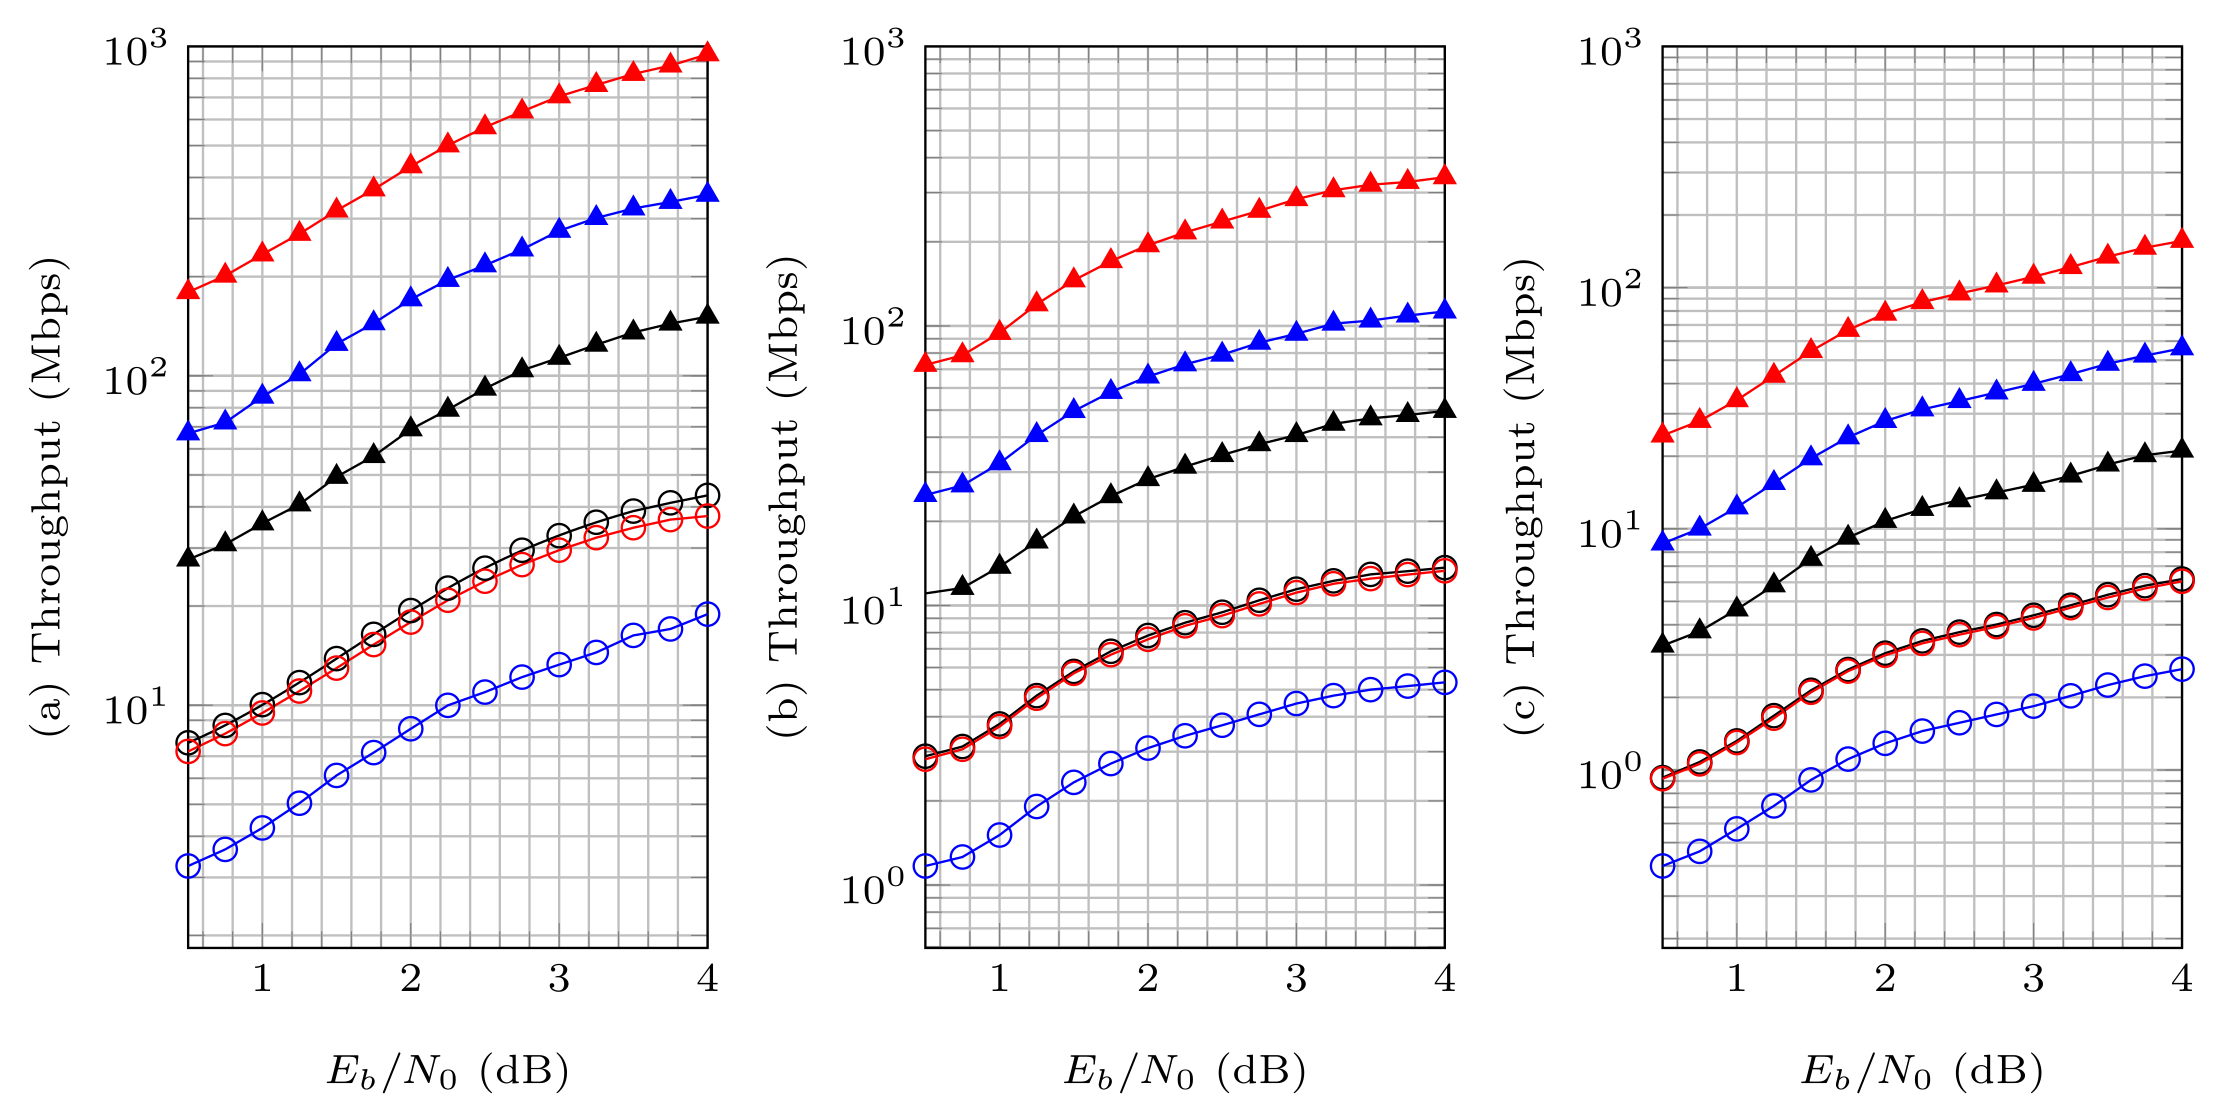
\includegraphics[width=\linewidth]{assets/fig5.png}
  \caption{
    启用提前停止准则时测量到的吞吐量:\\
    \textbf{a} $\mathbb{GF}(16)$ N=64 K=32的NB-LDPC码;
    \textbf{b} $\mathbb{GF}(64)$ N=384 K=192的NB-LDPC码;
    \textbf{c} $\mathbb{GF}(256)$ N=64 K=32的NB-LDPC码。\\
    圆圈曲线对应于单核实验,而三角形则对应于多核实验。
    $P_1$、$P_2$和$P_3$平台的结果分别用黑色、蓝色和红色绘制。
  }\label{fig:5}
\end{figure*}

  由于采用了提前停止准则,平均译码迭代次数明显减少,同时信噪比增大。这使得所提出的
  解码器的平均解码吞吐量增加。以平台$P_3$为例,当信噪比为3 dB且分配所有物理处理器核心时,
  对于$\mathbb{GF}(16)$、$\mathbb{GF}(64)$和$\mathbb{GF}(256)$的NB-LDPC码,
  吞吐量分别达到705 Mbps、284 Mbps和110 Mbps。

\section*{致谢}

致谢内容。


\nocite{*}

\bibliographystyle{cjc}
\bibliography{refs}



\appendix

\section{}

附录内容置于此处,字体为小5号宋体。附录内容包括:详细的定理证明、公式推导、原始数据等



% \begin{background}
% *论文背景介绍为英文,字体为小5号Times New Roman体*

% 论文后面为400单词左右的英文背景介绍。介绍的内容包括:

% 本文研究的问题属于哪一个领域的什么问题。该类问题目前国际上解决到什么程度。

% 本文将问题解决到什么程度。

% 课题所属的项目。

% 项目的意义。

% 本研究群体以往在这个方向上的研究成果。

% 本文的成果是解决大课题中的哪一部分,如果涉及863/973以及其项目、基金、研究计划,注意这些项目的英文名称应书写正确。
% \end{background}

\end{document}
